%% ----------------------------------------------------------------
%% Thesis.tex -- MAIN FILE (the one that you compile with LaTeX)
%% ---------------------------------------------------------------- 


% Set up the document
\documentclass[a4paper, 11pt, oneside]{Thesis}  % Use the "Thesis" style, based on the ECS Thesis style by Steve Gunn
\graphicspath{Figures/}  % Location of the graphics files (set up for graphics to be in PDF format)

% Include any extra LaTeX packages required
\usepackage[square, numbers, comma, sort&compress]{natbib}  % Use the "Natbib" style for the references in the Bibliography
\usepackage{verbatim}  % Needed for the "comment" environment to make LaTeX comments

\usepackage{algorithm}
\usepackage[noend]{algpseudocode}
\usepackage{pgfplots}
\usepackage{tikz}
\usetikzlibrary{shapes,arrows}
\usepackage{vector}  % Allows "\bvec{}" and "\buvec{}" for "blackboard" style bold vectors in maths
\hypersetup{urlcolor=blue, colorlinks=true}  % Colours hyperlinks in blue, but this can be distracting if there are many links.

%% ----------------------------------------------------------------
%\pgfplotsset{compat=1.15}
\begin{document}

\frontmatter      % Begin Roman style (i, ii, iii, iv...) page numbering

% Set up the Title Page
\title  {My Diary}

\authors  {\texorpdfstring
            {\href{183059001@iitb.ac.in}{Anand Chandrakant Pisal}\\{183059001}}
            {Author Name}
            }
\addresses  {\groupname\\\deptname\\\univname}  % Do not change this here, instead these must be set in the "Thesis.cls" file, please look through it instead
\date       {\today}
\subject    {}
\keywords   {}

\maketitle
%% ----------------------------------------------------------------


\setstretch{1.3}  % It is better to have smaller font and larger line spacing than the other way round

% Define the page headers using the FancyHdr package and set up for one-sided printing
\fancyhead{}  % Clears all page headers and footers
\rhead{\thepage}  % Sets the right side header to show the page number
\lhead{}  % Clears the left side page header

\pagestyle{fancy}  % Finally, use the "fancy" page style to implement the FancyHdr headers

%% ----------------------------------------------------------------
% Declaration Page required for the Thesis, your institution may give you a different text to place here

\begin{comment}
% The Abstract Page
\addtotoc{Abstract}  % Add the "Abstract" page entry to the Contents
\abstract{
\addtocontents{toc}{\vspace{1em}}  % Add a gap in the Contents, for aesthetics
Sentiment analysis is very important in extracting the sentiment behind the text, which can be mainly classified as positive, negative and neutral. With the growth of social media, sentiment analysis and opinion mining has become very helpful in identifying the opinion and sentiment and its related concepts such as sentiments, evaluations, attitudes and emotions and have wide application in product review, political survey, opinion polling etc. Positive or negative sentiment while sometimes depends on universally accepted positive or negative words, while sometimes it depends on positive or negative words under different topics. Topic modelling provides very useful tool in aspect based sentiment analysis. In this report we will take the journey from the creation of SENTIWORDNET, a lexical resource to sentiment analysis and opinion mining and go upto application of topic modelling for sentiment analysis, which based on different application helps in sentimental analysis.  
}
\end{comment}
\clearpage  % Abstract ended, start a new page
%% ----------------------------------------------------------------

\setstretch{1.3}  % Reset the line-spacing to 1.3 for body text (if it has changed)

% The Acknowledgements page, for thanking everyone

\begin{comment}
\acknowledgements{
\addtocontents{toc}{\vspace{1em}}  % Add a gap in the Contents, for aesthetics

I would like to acknowledge respected Prof. Pushpak Bhattacharya for his kind support  in guiding me the important concepts I need to go through for in depth concept of my research area. I would also like to acknowledge Aditya Joshi, who provide me necessary research papers for sentiment analysis. Also I am thankful to all the batchmates who encouraged me.

}
\clearpage  % End of the Acknowledgements
\end{comment}
%% ----------------------------------------------------------------

\pagestyle{fancy}  %The page style headers have been "empty" all this time, now use the "fancy" headers as defined before to bring them back


%% ----------------------------------------------------------------
%\lhead{\emph{Contents}}  % Set the left side page header to "Contents"
\tableofcontents  % Write out the Table of Contents

%\lhead{\emph{List of Figures}}  % Set the left side page header to "List if Figures"
\listoffigures  % Write out the List of Figures

%% ----------------------------------------------------------------
%\lhead{\emph{List of Tables}}  % Set the left side page header to "List of Tables"
\listoftables  % Write out the List of Tables



\addtocontents{toc}{\vspace{2em}}  % Add a gap in the Contents, for aesthetics


%% ----------------------------------------------------------------
\mainmatter	  % Begin normal, numeric (1,2,3...) page numbering
\pagestyle{fancy}  % Return the page headers back to the "fancy" style

% Include the chapters of the thesis, as separate files
% Just uncomment the lines as you write the chapters

\chapter{My classroom learning}
Dear Diary,

It was a wonderful experience for me to lot important things in the class. I would like
to share some the important things.

\section{Math class}
The equation of Latent Dirichlet allocation is very helpful in natural language processing
for modelling a generative statistical model. The equation of the model is shown below
:-

\begin{equation}
p(\beta ,\theta ,z,w|\alpha ,\eta )=\prod_{i=1}^{K}p(\beta _{i}|\eta )\prod_{d=1}^{D}p(\theta _{d},\alpha )(\prod_{n=1}^{N}p(z_{d,n}|\theta _{d})p(w_{d,n}|\beta _{1:K},z_{d,n}))
\end{equation}

Also the formula of cumulative distribution function in case of uniform probability measure is :-

\begin{equation}
F(x)=\begin{cases}
0, & \text{ if } x<a \\ 
\frac{x-a}{b-a}, & \text{ if } a\leq x\leq b \\ 
1, & \text{ if } x>b 
\end{cases}
\end{equation}

\section{Counting sort}
Counting sort is one of the nice algorithm which is not comparison based sorting. Below
is the counting sort algorithm :-

\begin{algorithm}
    \caption{Counting Sort}
    \begin{algorithmic}[1] % The number tells where the line numbering should start
        \Procedure{Counting-Sort}{$A,B,k$} 
        	\State Let C[0,...,k] be a new array
            \For{i=0\ to\ k :} 
                \State $C[i] = 0$ \Comment{Initialization step}
            \EndFor
            \For{j=1 to A.length or n :} 
                \State $C[A[j]] = C[A[j]] + 1$ \Comment{Maintaining count}
            \EndFor
            \For{i=1 to k:} 
                \State $C[i] = C[i] + C[i − 1]$
            \EndFor
            \For{j=n or A.length down to 1:} 
                \State $B[C[A[j]]] = A[j]$
				\State $C[A[j]] = C[A[j]] − 1$
            \EndFor
        \EndProcedure
    \end{algorithmic}
\end{algorithm}
 % Introduction

\chapter{Watched Cricket match}
India and Australia match is always wonderful to watch. While Australia was 170/10
in 17.4 over, India scored 172/4 in 15.5 over and won by 6 wickets.

Below is the line graph.

\begin{figure}[H]
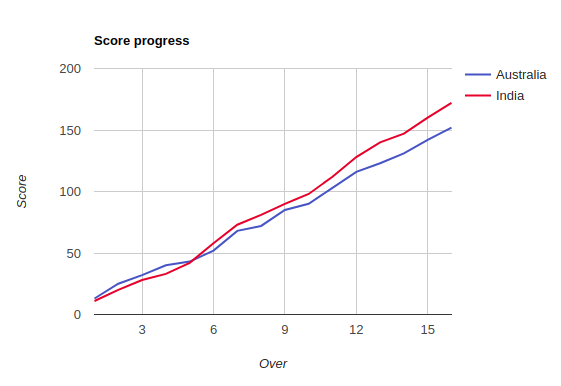
\includegraphics[scale=0.5]{line_graph.png}
\caption{Line graph of India Vs Australia}
\end{figure}

Also the bar graph was like shown in figure 2.2 :-

\pgfplotstableread[row sep=\\,col sep=&]{
    over & aus 	& india	\\
    1    & 	13 	&	11 	\\
    2    & 	12  & 	9 	\\
    3    & 	7 	& 	8 	\\
    4    & 	8 	& 	5 	\\
    5    & 	3  	& 	9 	\\
    6    & 	9  	& 	16 	\\
    7	 &	16	&	15	\\
    8	 &	4	&	8	\\
    9	 &	13	&	9	\\
    10	 &	5	&	8	\\
    11	 &	13	&	14	\\
    12	 &	13	&	16	\\
    13	 &	7	&	12	\\
    14	 &	8	&	7	\\
    15	 &	11	&	13	\\
    16	 & 	10	&	12	\\
    17	 &	7	&	0	\\
    18	 &	11 	&	0	\\
    }\mydata

\begin{figure}
\begin{tikzpicture}
    \begin{axis}[
            ybar,          
            bar width=.2cm,
            width=\textwidth,
            height=.5\textwidth,
            legend style={at={(0.5,1)},
                anchor=north,legend columns=-1},  
            symbolic x coords={1,2,3,4,5,6,7,8,9,10,11,12,13,14,15,16,17,18},
        ]
        \addplot table[x=over,y=aus]{\mydata};
        \addplot table[x=over,y=india]{\mydata};
        \legend{Australia,India}
    \end{axis}
\end{tikzpicture}
\caption{Bar graph of India Vs Australia}
\end{figure} % Background Theory 

\chapter{Miscellaneous activity}

\section{My semester expense}
I want to prepare my semester expense falling mainly into below categories:-
\\

\textbf{Semester fee} This include my tution fee

\textbf{Mess expense} My mess fee.

\textbf{Stationary} My stationary requirement

\textbf{Transportation} Mainly include my home trip

\textbf{Entertainment} Very less, because I am student of IIT Bombay

\textbf{Miscellaneous} Other important things
\\

Below table describe my expanse:-


\begin{table}[h!]
  \begin{center}
    \begin{tabular}{|p{4cm}|p{4cm}|}
      \hline
      \multicolumn{2}{|c|}{Per semester Expanse}\\
      \hline
      Expanse due to & Amount\\
	  \hline      
	  Semester fee & 18000\\
	  Mess expense & 20000\\
	  Stationary & 7000\\
	  Transportation & 9000\\
	  Entertainment & 5000\\
	  Miscellaneous & 4000\\
	\hline    
    \end{tabular}
    \caption{My semester expanse}
  \end{center}
\end{table}

\section{My favorite recipe}
I like to learn new cooking item. I went through recipe of preparing stuff for aloo
paratha. Below is the recipe.

\tikzstyle{startstop} = [ellipse, text centered, draw=black, fill=red!20]
\tikzstyle{process} = [rectangle, rounded corners, text width=2cm,text centered, draw=black, fill=blue!20]
\tikzstyle{decision} = [diamond, text centered, text width=2cm, draw=black, fill=blue!20]
\tikzstyle{arrow} = [thick,->,>=stealth]

\begin{figure}[h!]
\begin{center}
\begin{tikzpicture}[node distance=2cm]
\node (start) [startstop] {Start};
\node (pro1) [process, below of=start] {Boil potato in pressure cooker};
\node (pro2) [process, below of=pro1, yshift=-1cm] {Mash The potato nicely};
\node (pro3) [process, left of=pro2, xshift=-1.5cm] {Add little water};
\node (dec) [decision, below of=pro2, yshift=-1.5cm] {Has the mash softend};
\node (pro4) [process, right of=dec, xshift=3cm] {Mix with the other spices};
\node (pro5) [process, below of=dec, yshift=-2cm] {Stuff is ready for preparing Aloo Paratha};
\node (end) [startstop, below of=pro5, yshift=-0.5cm] {End};
\draw [arrow] (start) -- (pro1);
\draw [arrow] (pro1) -- (pro2);
\draw [arrow] (pro2) -- (dec);
\draw [arrow] (pro3) -- (pro2);
\draw [arrow] (dec) -| node[anchor=east] {No} (pro3);
\draw [arrow] (dec) -- node[anchor=south] {Yes} (pro4);
\draw [arrow] (pro4) |- (pro5);
\draw [arrow] (pro5) -- (end);
\end{tikzpicture}
\end{center}
\caption{Stuff preparation of Aloo Paratha}
\end{figure}

\section{Some important research ideas.}
Paper\cite{arxivPreprint} describes how word embedding helps in sarcasm detection by augmenting
the word embedding-based features to the sets of features of sarcasm. Similarity score
values returned by word embeddings, are of two categories:- similarity-based (where we consider maximum/minimum similarity score of most similar/dissimilar word pair
respectively), and weighted similarity-based (where we weight the maximum/minimum
similarity scores of most similar/dissimilar word pairs with the linear distance between
the two words in the sentence).

Paper\cite{acmSurvey} is a compilation of past work in automatic sarcasm detection. The three
milestones observed in the research so far: semi-supervised pattern extraction to iden-
tify implicit sentiment, use of hashtag-based supervision, and incorporation of context
beyond target text.

 % Experimental Setup



%% ----------------------------------------------------------------
% Now begin the Appendices, including them as separate files

\addtocontents{toc}{\vspace{2em}} % Add a gap in the Contents, for aesthetics

%\appendix % Cue to tell LaTeX that the following 'chapters' are Appendices



\begin{thebibliography}{1}

\bibitem{arxivPreprint}
Joshi, Aditya, et al. ''Are Word Embedding-based Features Useful for Sarcasm Detection?.'' arXiv preprint arXiv:1610.00883 (2016).
  
\bibitem{acmSurvey}
Joshi, Aditya, Pushpak Bhattacharyya, and Mark J. Carman.  ''Automatic sarcasm detection: A survey.'' ACM Computing Surveys (CSUR) 50.5 (2017): 73.

\end{thebibliography}
	% Appendix Title

%\input{Appendices/AppendixB} % Appendix Title

%\input{Appendices/AppendixC} % Appendix Title

\addtocontents{toc}{\vspace{2em}}  % Add a gap in the Contents, for aesthetics
\backmatter

%% ----------------------------------------------------------------


\end{document}  % The End
%% ----------------------------------------------------------------
\grid
\grid
